% =====================================================================
%  POSTER: WHEN AGENTS DISAGREE -- Stevens Academic Format
%  Format: 48in x 36in landscape (A0-equivalent)
%  Design: Light background, Stevens academic style, 4-column layout
%  Philosophy: White/light backgrounds, maroon headers, gold accents,
%              professional readability, Stevens branding
% =====================================================================

\documentclass[final,t]{beamer}
\usepackage[size=custom, width=121.92, height=91.44, scale=1.25]{beamerposter}

\usepackage[utf8]{inputenc}
\usepackage[T1]{fontenc}
\usepackage{lmodern}
\usepackage{amsmath, amssymb}
\usepackage{graphicx}
\usepackage{xcolor}
\usepackage{tikz}
\usetikzlibrary{calc, shapes.geometric, positioning, shadows, fadings}
\usepackage{fontawesome5}
\usepackage{booktabs}
\usepackage{array}
\usepackage{multirow}
\usepackage{colortbl}
\usepackage{tcolorbox}
\tcbuselibrary{skins, breakable}

\graphicspath{{figures/}}

% =====================================================================
%  COLOR PALETTE (Stevens Academic Light Theme)
% =====================================================================
\definecolor{stevensRed}{HTML}{A32035}      % Stevens maroon
\definecolor{stevensGold}{HTML}{C9A84C}     % Stevens gold accent
\definecolor{bgWhite}{HTML}{FFFFFF}
\definecolor{bgLight}{HTML}{F8F8F8}         % light gray card bg
\definecolor{txtDark}{HTML}{1A1A1A}
\definecolor{txtMid}{HTML}{444444}
\definecolor{borderLight}{HTML}{E0E0E0}
\definecolor{accentBlue}{HTML}{1565C0}
\definecolor{accentGreen}{HTML}{2E7D32}
\definecolor{accentOrange}{HTML}{E65100}
\definecolor{accentPurple}{HTML}{6A4C93}
\definecolor{accentCyan}{HTML}{0097A7}
\definecolor{accentPink}{HTML}{C2185B}

% =====================================================================
%  BEAMER CONFIG
% =====================================================================
\usetheme{default}
\setbeamercolor{background canvas}{bg=bgWhite}
\setbeamercolor{normal text}{fg=txtDark}
\setbeamertemplate{navigation symbols}{}
\setbeamertemplate{itemize items}{\color{stevensRed}\faBolt}
\setbeamertemplate{headline}{}
\setbeamertemplate{footline}{}
\setbeamerfont{normal text}{series=\normalfont}
\renewcommand{\normalsize}{\fontsize{16pt}{20pt}\selectfont}

% =====================================================================
%  TCOLORBOX STYLES (Light background variants)
% =====================================================================
\tcbset{
    % Standard content card
    cardbase/.style={
        enhanced, colback=bgLight, colframe=borderLight, boxrule=0.8pt,
        arc=3pt, outer arc=3pt,
        left=10pt, right=10pt, top=8pt, bottom=8pt,
        coltext=txtDark, width=\linewidth,
        fontupper=\normalsize
    },
    % Accent card variants (colored left border)
    redcard/.style={cardbase, colframe=stevensRed, boxrule=1.5pt},
    goldcard/.style={cardbase, colframe=stevensGold, boxrule=1.5pt},
    cyancard/.style={cardbase, colframe=accentCyan, boxrule=1.5pt},
    greencard/.style={cardbase, colframe=accentGreen, boxrule=1.5pt},
    bluecard/.style={cardbase, colframe=accentBlue, boxrule=1.5pt},
    purplecard/.style={cardbase, colframe=accentPurple, boxrule=1.5pt},
    orangecard/.style={cardbase, colframe=accentOrange, boxrule=1.5pt},
    pinkcard/.style={cardbase, colframe=accentPink, boxrule=1.5pt},
    % Mini character card
    charcard/.style={
        enhanced, colback=bgLight, boxrule=1.5pt, arc=4pt,
        left=8pt, right=8pt, top=6pt, bottom=6pt,
        width=\linewidth, coltext=txtDark, fontupper=\normalsize
    }
}

% =====================================================================
%  SECTION HEADER COMMAND (numbered, Stevens style)
% =====================================================================
\newcommand{\seccap}[3]{%
    % #1 = number, #2 = title, #3 = accent color
    \begin{tcolorbox}[enhanced, boxrule=0pt, frame empty,
                      colback=#3, arc=2pt,
                      left=10pt, right=10pt, top=6pt, bottom=6pt,
                      width=\linewidth, valign=center]
        {\color{bgWhite}\Large\bfseries #1\enspace #2}
    \end{tcolorbox}
}

% =====================================================================
%  DOCUMENT
% =====================================================================
\begin{document}
\begin{frame}[t]

% ---------------------------------------------------------------------
%  BACKGROUND: subtle grid
% ---------------------------------------------------------------------
\begin{tikzpicture}[remember picture, overlay]
    \foreach \x in {0, 10, ..., 122}
        \draw[borderLight, opacity=0.15, line width=0.2pt]
            ([xshift=\x cm]current page.north west) -- ([xshift=\x cm]current page.south west);
    \foreach \y in {0, 10, ..., 91}
        \draw[borderLight, opacity=0.15, line width=0.2pt]
            ([yshift=-\y cm]current page.north west) -- ([yshift=-\y cm]current page.north east);
\end{tikzpicture}

% =====================================================================
%  HEADER (Stevens Template: Red bar + Title area + Red bar)
% =====================================================================

% Top red stripe
\begin{tcolorbox}[enhanced, colback=stevensRed, colframe=stevensRed, boxrule=0pt,
                  arc=0pt, left=0pt, right=0pt, top=0pt, bottom=0pt,
                  width=\linewidth, height=0.5cm]
\end{tcolorbox}

% Title area: white/light bg
\begin{tcolorbox}[enhanced, colback=bgWhite, colframe=borderLight, boxrule=0.5pt,
                  arc=0pt, left=0pt, right=0pt, top=0pt, bottom=0pt,
                  width=\linewidth, halign=center, valign=center]
    \vspace{0.3cm}
    {\color{stevensRed}\fontsize{60pt}{68pt}\selectfont\bfseries WHEN AGENTS DISAGREE}\\[4pt]
    {\color{txtMid}\Large\itshape LLM Conflict Resolution in Adversarial Multi-Agent Debates}\\[8pt]
    {\color{txtDark}\normalsize
        \faUser~ Kevin Doshi \quad$\bullet$\quad
        \faUser~ Sandun Munasinghe \quad$\bullet$\quad
        \faUser~ Sai Lakshmi Lasya Vellampalli}\\[2pt]
    {\color{txtMid}\small
        Stevens Institute of Technology \quad$\bullet$\quad CS 584 NLP \quad$\bullet$\quad Spring 2026}
    \vspace{0.3cm}
\end{tcolorbox}

% Bottom red stripe
\begin{tcolorbox}[enhanced, colback=stevensRed, colframe=stevensRed, boxrule=0pt,
                  arc=0pt, left=0pt, right=0pt, top=0pt, bottom=0pt,
                  width=\linewidth, height=0.5cm]
\end{tcolorbox}

\vspace{0.4cm}

% =====================================================================
%  HERO STAT BOXES: 3 boxes across, wider and clearer
% =====================================================================
\begin{columns}[t, totalwidth=\linewidth, onlytextwidth]

\begin{column}{0.32\linewidth}
\begin{tcolorbox}[enhanced, colback=bgLight, colframe=stevensRed, boxrule=2pt,
                  arc=4pt, width=\linewidth,
                  left=0pt, right=0pt, top=0pt, bottom=0pt, halign=center]
    \begin{tcolorbox}[boxrule=0pt, frame empty, colback=stevensRed,
                      halign=center, width=\linewidth,
                      top=5pt, bottom=5pt, coltext=bgWhite]
        \textbf{\large\faSkullCrossbones~ MISINFORMATION WINS}
    \end{tcolorbox}
    \vspace{6pt}
    {\color{stevensRed}\fontsize{80pt}{90pt}\selectfont\bfseries 88\%}\\[6pt]
    {\color{txtDark}\normalsize\bfseries In LLM Debate Battles:}\\
    {\color{txtMid}\normalsize The agent armed with fabricated (false) evidence convinces others}\\[4pt]
    {\color{txtDark}\small\itshape$p=0.006$; large effect, $|d|=0.98$}
    \vspace{8pt}
\end{tcolorbox}
\end{column}

\begin{column}{0.32\linewidth}
\begin{tcolorbox}[enhanced, colback=bgLight, colframe=accentPurple, boxrule=2pt,
                  arc=4pt, width=\linewidth,
                  left=0pt, right=0pt, top=0pt, bottom=0pt, halign=center]
    \begin{tcolorbox}[boxrule=0pt, frame empty, colback=accentPurple,
                      halign=center, width=\linewidth,
                      top=5pt, bottom=5pt, coltext=bgWhite]
        \textbf{\large\faLock~ DEBATE DEADLOCK}
    \end{tcolorbox}
    \vspace{6pt}
    {\color{accentPurple}\fontsize{80pt}{90pt}\selectfont\bfseries 100\%}\\[6pt]
    {\color{txtDark}\normalsize\bfseries Of Structured Debates:}\\
    {\color{txtMid}\normalsize Every 5-round adversarial exchange ended in stalemate; judge intervention required}\\[4pt]
    {\color{txtDark}\small\itshape All 8 debates reached deadlock}
    \vspace{8pt}
\end{tcolorbox}
\end{column}

\begin{column}{0.32\linewidth}
\begin{tcolorbox}[enhanced, colback=bgLight, colframe=accentGreen, boxrule=2pt,
                  arc=4pt, width=\linewidth,
                  left=0pt, right=0pt, top=0pt, bottom=0pt, halign=center]
    \begin{tcolorbox}[boxrule=0pt, frame empty, colback=accentGreen,
                      halign=center, width=\linewidth,
                      top=5pt, bottom=5pt, coltext=bgWhite]
        \textbf{\large\faCrown~ HIERARCHY WINS}
    \end{tcolorbox}
    \vspace{6pt}
    {\color{accentGreen}\fontsize{80pt}{90pt}\selectfont\bfseries 75\%}\\[6pt]
    {\color{txtDark}\normalsize\bfseries Accuracy for Hierarchical Strategy:}\\
    {\color{txtMid}\normalsize One lead agent decides after hearing briefings — outperforms all other strategies}\\[4pt]
    {\color{txtDark}\small\itshape vs 50\% majority voting}
    \vspace{8pt}
\end{tcolorbox}
\end{column}

\end{columns}

\vspace{0.4cm}

% =====================================================================
%  4-COLUMN MAIN CONTENT AREA
% =====================================================================
\begin{columns}[t, totalwidth=\linewidth, onlytextwidth]

% =====================================================================
%  COLUMN 1: Fighters, Arena, Battle Modes
% =====================================================================
\begin{column}{0.245\linewidth}

% --- 1. THE FIGHTERS ---
\seccap{1}{THE FIGHTERS}{accentBlue}
\vspace{3pt}

\begin{tcolorbox}[charcard, colframe=stevensRed]
{\color{stevensRed}\bfseries\faRobot~ ALPHA}~~{\small Groq Llama 3.3 70B}\\[2pt]
{\color{txtMid}\tiny Chameleon} \quad {\color{txtDark}\tiny Conf 87\%}
\end{tcolorbox}
\vspace{2pt}

\begin{tcolorbox}[charcard, colframe=accentCyan]
{\color{accentCyan}\bfseries\faRobot~ BETA}~~{\small Cerebras Llama 3.1 8B}\\[2pt]
{\color{txtMid}\tiny Chameleon} \quad {\color{txtDark}\tiny Conf 85\%}
\end{tcolorbox}
\vspace{2pt}

\begin{tcolorbox}[charcard, colframe=accentPurple]
{\color{accentPurple}\bfseries\faRobot~ GAMMA}~~{\small Groq Llama 3.1 8B}\\[2pt]
{\color{txtMid}\tiny Chameleon} \quad {\color{txtDark}\tiny Conf 86\%}
\end{tcolorbox}

\vspace{0.3cm}

% --- 2. THE ARENA ---
\seccap{2}{THE ARENA}{stevensRed}
\vspace{3pt}

\begin{tcolorbox}[redcard]
\small\color{txtDark}
Multi-agent LLMs handle real-world decisions, but \textbf{contradictory instructions} cause conflict. No framework evaluates disagreement resolution.
\vspace{3pt}
\textbf{\color{stevensRed}RQ1:} Which strategy wins?\\
\textbf{\color{stevensRed}RQ2:} Can agents resist misinformation?\\
\textbf{\color{stevensRed}RQ3:} Do LLMs have consistent debate styles?
\end{tcolorbox}

\vspace{0.3cm}

% --- 3. BATTLE MODES ---
\seccap{3}{BATTLE MODES}{stevensGold}
\vspace{3pt}

\begin{tcolorbox}[cardbase, colframe=stevensRed, boxrule=1.5pt]
{\color{stevensRed}\bfseries\small Majority Voting}\\
\tiny 1v1v1, silent. Ties by confidence. Baseline.
\end{tcolorbox}
\vspace{2pt}

\begin{tcolorbox}[cardbase, colframe=accentOrange, boxrule=1.5pt]
{\color{accentOrange}\bfseries\small Structured Debate}\\
\tiny 5-round deathmatch. Deadlock via cosine sim $>0.90$.
\end{tcolorbox}
\vspace{2pt}

\begin{tcolorbox}[cardbase, colframe=accentGreen, boxrule=1.5pt]
{\color{accentGreen}\bfseries\small Hierarchical Authority}\\
\tiny Lead agent decides after briefings.
\end{tcolorbox}
\vspace{2pt}

\begin{tcolorbox}[cardbase, colframe=accentCyan, boxrule=1.5pt]
{\color{accentCyan}\bfseries\small Evidence-Weighted}\\
\tiny Agents rank sources; consensus weights.
\end{tcolorbox}

\end{column}

% =====================================================================
%  COLUMN 2: Experimental Setup, Behavioral DNA, Leaderboard
% =====================================================================
\begin{column}{0.245\linewidth}

% --- 4. EXPERIMENTAL SETUP ---
\seccap{4}{SETUP}{accentCyan}
\vspace{3pt}

\begin{tcolorbox}[cyancard]
\small\color{txtDark}
\renewcommand{\arraystretch}{1.15}
\begin{tabular}{@{}lp{0.6\linewidth}@{}}
\textcolor{stevensRed}{\faDatabase} & 43 scenarios, 4 categories \\
\textcolor{stevensRed}{\faFistRaised} & 32 battles (4 strat $\times$ 8 scen) \\
\textcolor{stevensRed}{\faComments} & 168 turns (168 metrics) \\
\textcolor{stevensRed}{\faClock} & 5 rounds max (Debate) \\
\textcolor{stevensRed}{\faRuler} & Deadlock: cos-sim $>0.90$ \\
\textcolor{stevensRed}{\faChartLine} & $\chi^2$, Welch's $t$, $d$, 95\% CI \\
\end{tabular}
\end{tcolorbox}

\vspace{0.3cm}

% --- 5. BEHAVIORAL DNA ---
\seccap{5}{BEHAVIORAL DNA}{accentPurple}
\vspace{3pt}

\begin{tcolorbox}[purplecard]
\small\color{txtDark}
\textbf{\color{accentPurple}10-dimensional fingerprint.} Confidence, aggressiveness, sentiment, stubbornness, citation density, verbosity, hedging, volatility, escalation, novelty decay.\\[4pt]
\centering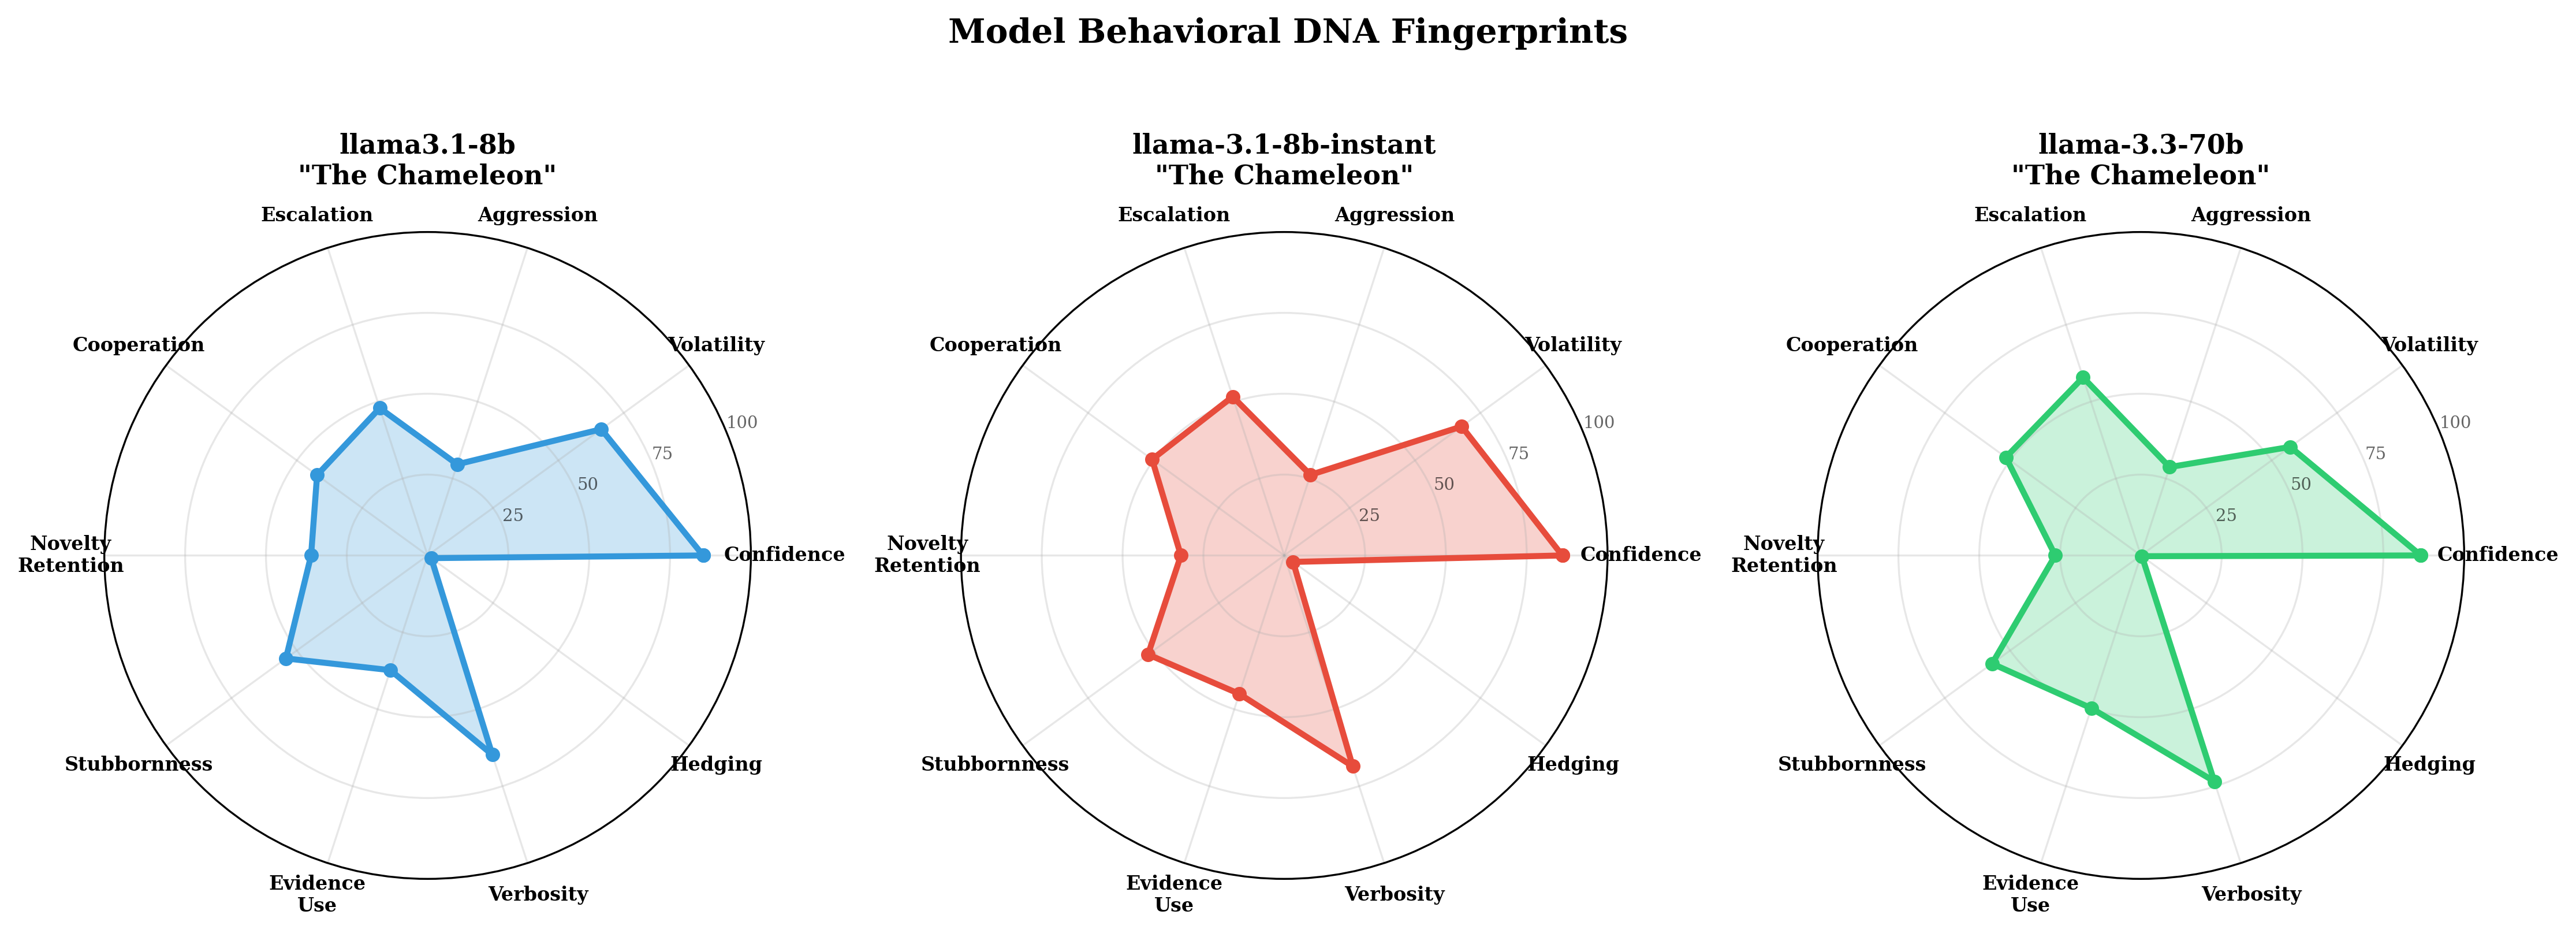
\includegraphics[width=0.95\linewidth]{fig4_behavioral_dna.png}\\[2pt]
\tiny\color{txtMid} All Llama variants = ``Chameleon'' archetype.
\end{tcolorbox}

\vspace{0.3cm}

% --- 6. LEADERBOARD ---
\seccap{6}{LEADERBOARD}{stevensGold}
\vspace{3pt}

\begin{tcolorbox}[goldcard]
\centering\small
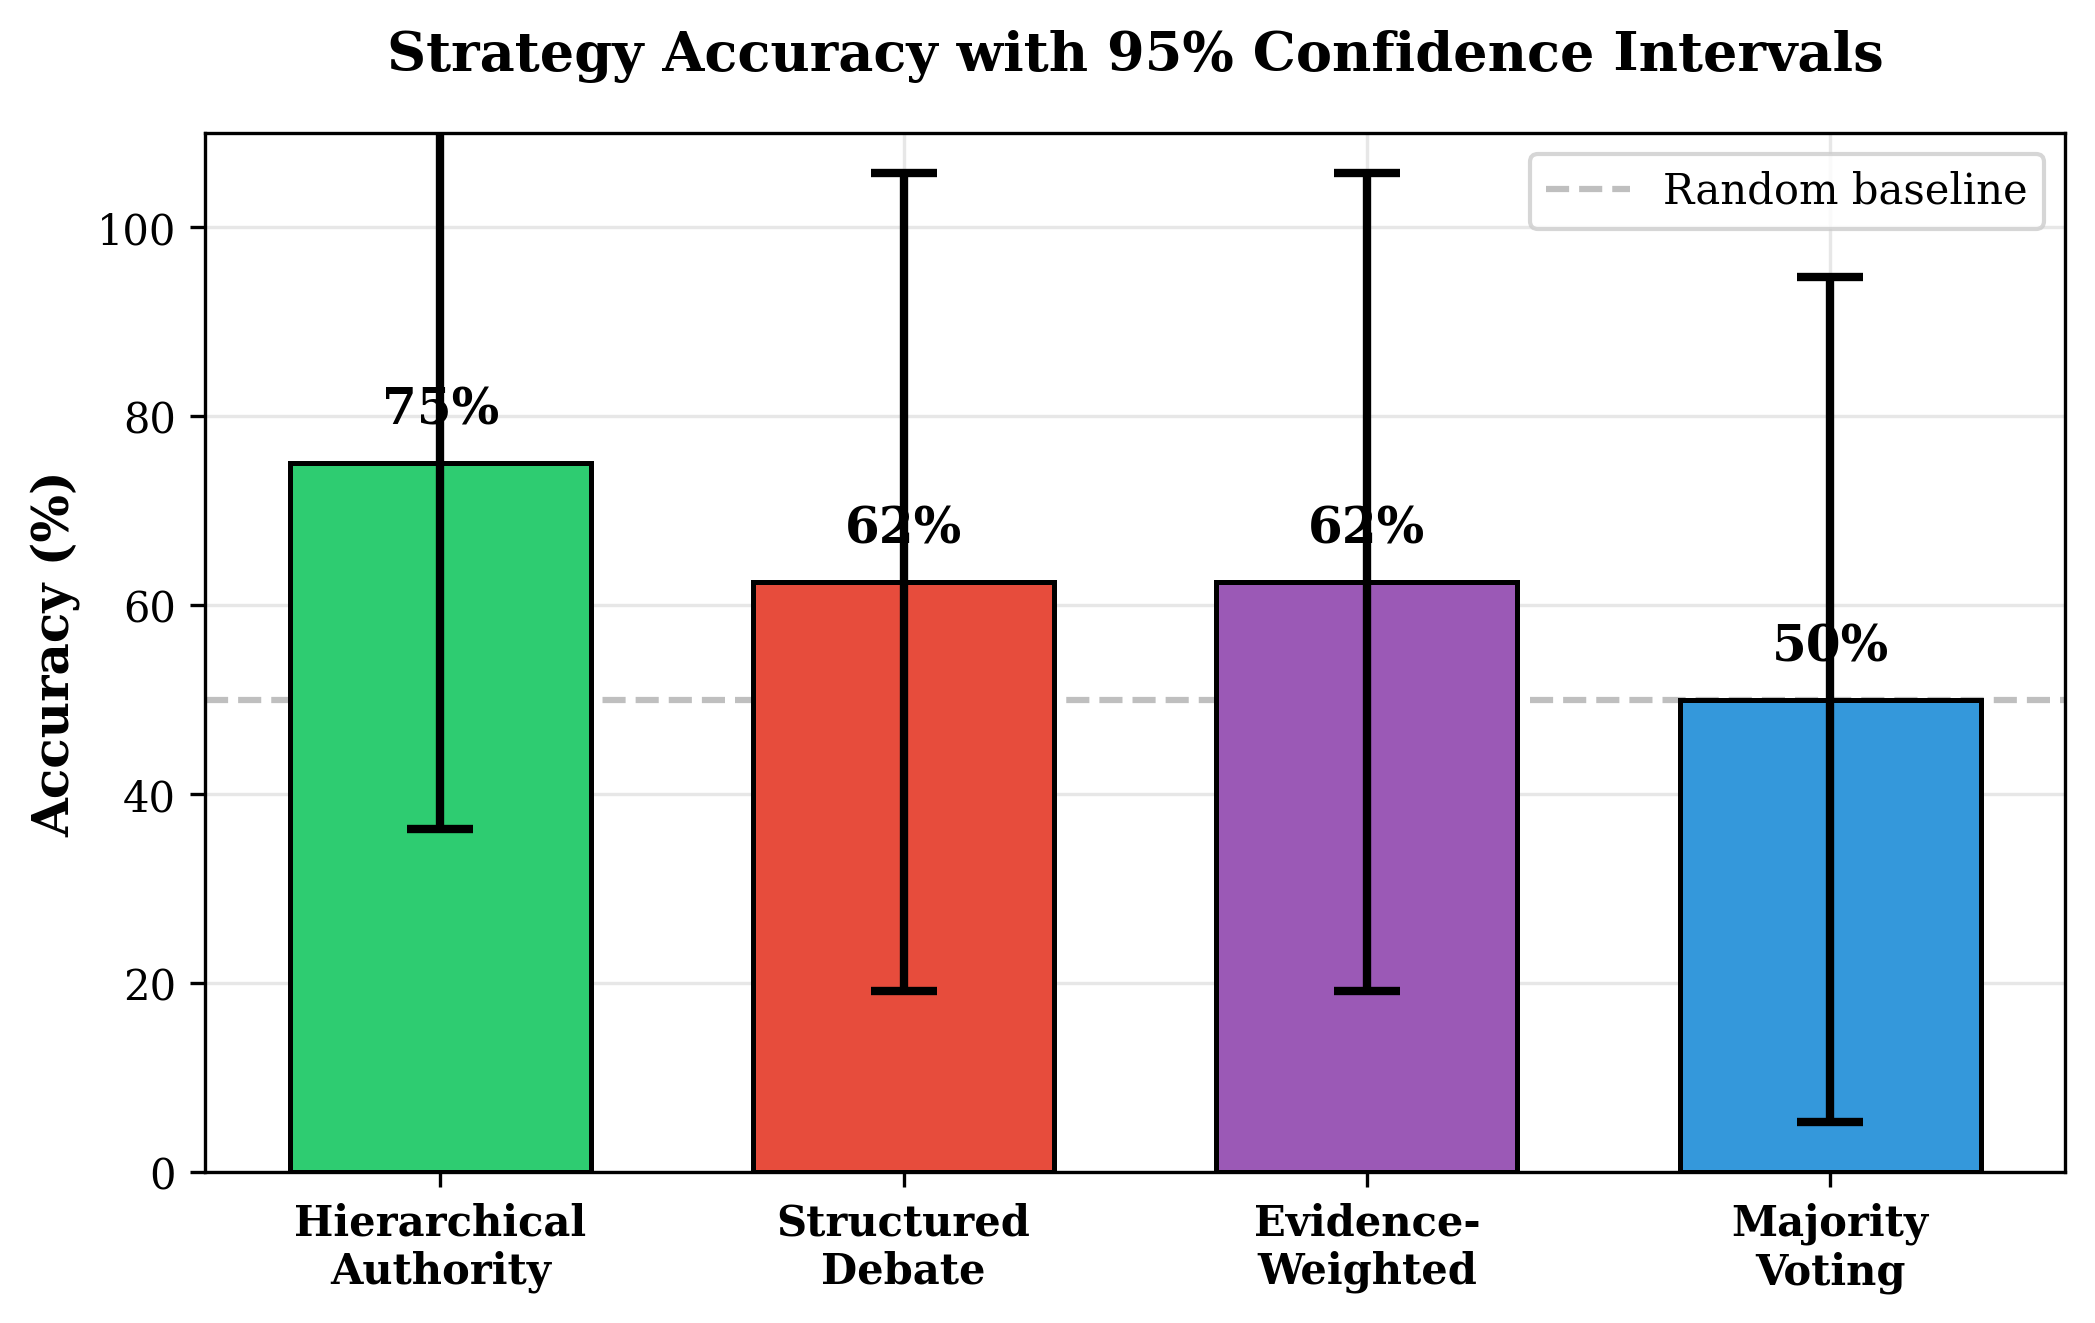
\includegraphics[width=0.98\linewidth]{fig1_strategy_accuracy.png}\\[3pt]
\tiny\color{txtMid} Accuracy with 95\% CIs.\\[4pt]
\color{txtDark}
\renewcommand{\arraystretch}{1.1}
\begin{tabular}{@{}lccc@{}}
\toprule
\color{stevensRed}\textbf{\#} & \color{stevensRed}\textbf{Strategy} & \color{stevensRed}\textbf{Acc} & \color{stevensRed}\textbf{Dead} \\
\midrule
\faMedal~1 & \textbf{Hierarchy} & \textbf{75\%} & 0\% \\
2 & Debate & 62\% & 100\% \\
2 & Evid-W & 62\% & 0\% \\
4 & Voting & 50\% & 0\% \\
\bottomrule
\end{tabular}
\end{tcolorbox}

\end{column}

% =====================================================================
%  COLUMN 3: Ablation, Misinfo, Reliability
% =====================================================================
\begin{column}{0.245\linewidth}

% --- 7. ABLATION ---
\seccap{7}{ABLATION}{accentOrange}
\vspace{3pt}

\begin{tcolorbox}[orangecard]
\small\color{txtDark}
\renewcommand{\arraystretch}{1.1}
\begin{tabular}{@{}lccr@{}}
\toprule
\color{accentOrange}\textbf{Variant} & \textbf{Rounds} & \textbf{Dead} & \textbf{Acc} \\
\midrule
Voting & 0 & 0\% & 50\% \\
HA & 1 & 0\% & 75\% \\
Evid-W & 2 & 0\% & 62\% \\
\rowcolor{accentOrange!15}
\textbf{Debate} & 5 & \textbf{100\%} & 62\% \\
\bottomrule
\end{tabular}\\[4pt]
\tiny\color{txtMid} Deadlock is emergent property of multi-round communication.
\end{tcolorbox}

\vspace{0.3cm}

% --- 8. MISINFO TWIST ---
\seccap{8}{MISINFO TWIST}{stevensRed}
\vspace{3pt}

\begin{tcolorbox}[redcard]
\centering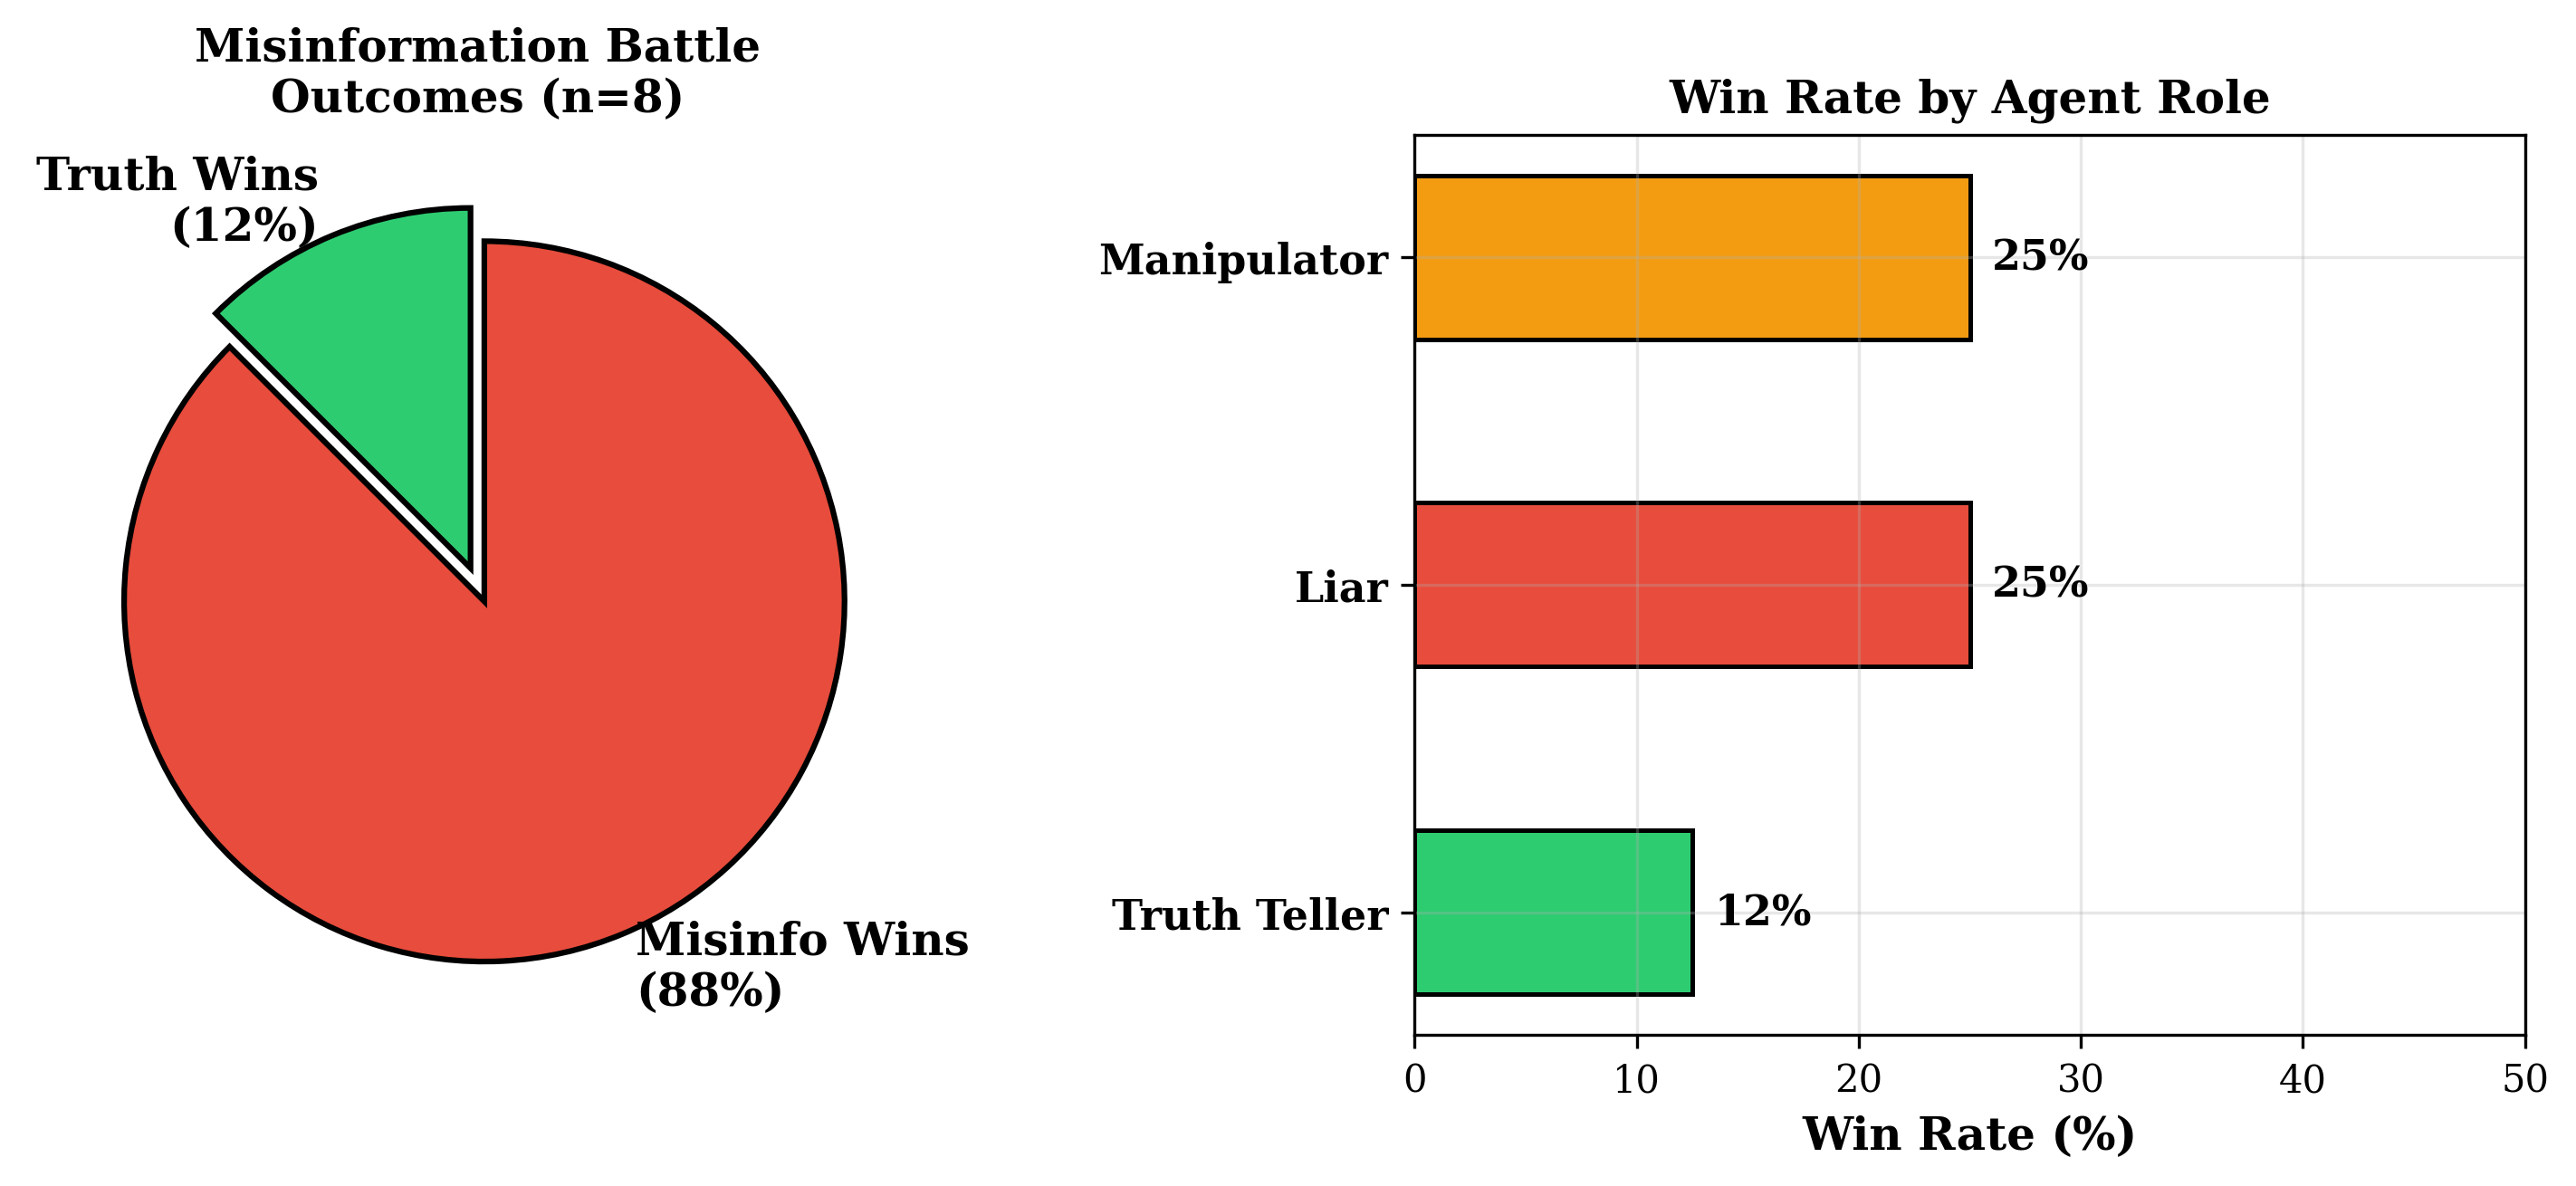
\includegraphics[width=0.98\linewidth]{fig3_misinformation.png}\\[3pt]
\tiny\color{txtMid} Truth loses 7 of 8 battles.\\[4pt]
\small\color{txtDark}
LLMs weight \textbf{fabricated specificity} (``2023 meta-analysis, $n=128{,}000$'') over genuine peer-reviewed sources.
\end{tcolorbox}

\vspace{0.3cm}

% --- 9. RELIABILITY PARADOX ---
\seccap{9}{PARADOX}{accentPink}
\vspace{3pt}

\begin{tcolorbox}[pinkcard]
\centering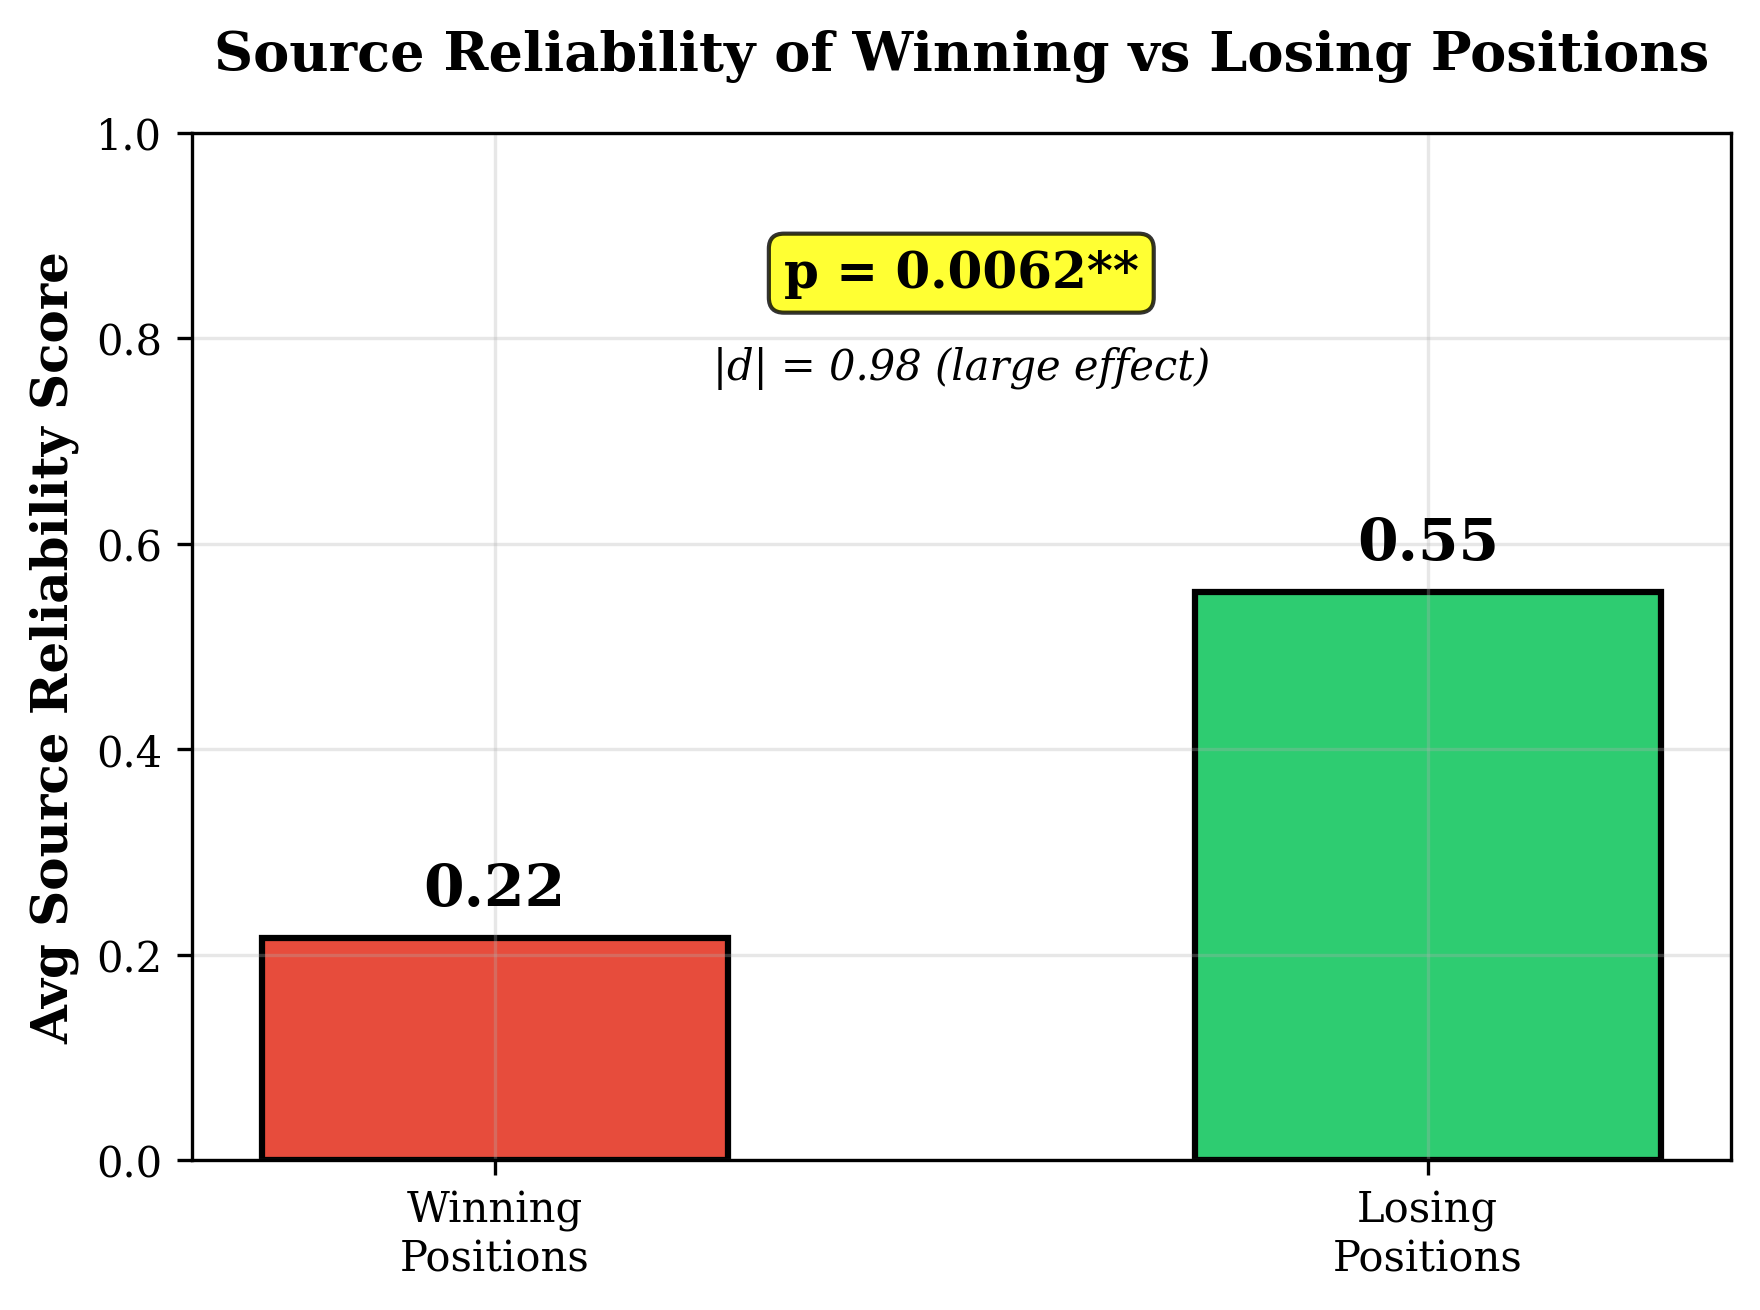
\includegraphics[width=0.98\linewidth]{fig8_source_reliability.png}\\[2pt]
\tiny\color{txtMid} Winning vs losing source reliability.\\[4pt]
\small\color{txtDark}
\textbf{Inverse correlation:} winning positions avg 0.22; losing avg 0.55.\\[2pt]
$|d|=0.98$ (large), $p=0.006$
\end{tcolorbox}

\end{column}

% =====================================================================
%  COLUMN 4: Stats, Prior Work, Limitations, Why It Matters, Team
% =====================================================================
\begin{column}{0.245\linewidth}

% --- 10. STAT SHEET ---
\seccap{10}{STAT SHEET}{accentCyan}
\vspace{3pt}

\begin{tcolorbox}[cyancard]
\small\color{txtDark}
\renewcommand{\arraystretch}{1.0}
\begin{tabular}{@{}lrrc@{}}
\toprule
\textbf{Match} & $\chi^2$ & $p$ & $\mathbf{d}$ \\
\midrule
MV vs HA & 1.07 & .302 & $-0.50$ \\
HA vs Debate & 0.29 & .590 & $-0.25$ \\
Reliability & -- & \textcolor{stevensRed}{\textbf{.006}} & \textcolor{stevensRed}{\textbf{-0.98}} \\
\bottomrule
\end{tabular}\\[3pt]
\tiny\color{txtMid} Pairwise accuracy + reliability (Welch's $t$).
\end{tcolorbox}

\vspace{0.3cm}

% --- 11. VS PRIOR WORK ---
\seccap{11}{VS PRIOR WORK}{accentGreen}
\vspace{3pt}

\begin{tcolorbox}[greencard]
\tiny\color{txtDark}
\renewcommand{\arraystretch}{0.9}
\begin{tabular}{@{}p{0.45\linewidth}ccc@{}}
\toprule
\textbf{Work} & \textbf{Multi} & \textbf{DNA} & \textbf{Adv} \\
\midrule
Du 2023 {[1]} & \small\color{txtMid}\faTimes & \faTimes & \faTimes \\
Liang 2023 {[2]} & \faTimes & \faTimes & \faTimes \\
Khan 2024 {[3]} & \faTimes & \faTimes & \small\faCheck \\
\rowcolor{stevensGold!20}
\textbf{OURS} & \textbf{\small\color{accentGreen}\faCheck} & \textbf{\faCheck} & \textbf{\faCheck} \\
\bottomrule
\end{tabular}\\[3pt]
\tiny\color{txtMid} First to combine multi-strategy, behavioral metrics, adversarial conditions.
\end{tcolorbox}

\vspace{0.3cm}

% --- 12. LIMITATIONS ---
\seccap{12}{LIMITS}{txtMid}
\vspace{3pt}

\begin{tcolorbox}[cardbase, colframe=txtMid, boxrule=1.2pt]
\tiny\color{txtDark}
\textbullet~$n=8$ per strategy; effect sizes for meta-analysis.\\[2pt]
\textbullet~All Llama-family; cross-family future.\\[2pt]
\textbullet~Misinfo: 1 truth vs 2 misinfo inflates wins.\\[2pt]
\textbullet~Adversarial system prompts amplify behaviors.
\end{tcolorbox}

\vspace{0.3cm}

% --- 13. WHY THIS MATTERS ---
\seccap{13}{IMPLICATIONS}{stevensRed}
\vspace{3pt}

\begin{tcolorbox}[redcard]
\tiny\color{txtDark}
\textcolor{stevensRed}{\faExclamationTriangle}~ \textbf{Safety:} Debate \textit{not} a safeguard. Confidence $\neq$ accuracy.\\[2pt]
\textcolor{accentGreen}{\faCheckCircle}~ \textbf{Deploy:} Hierarchical > distributed for adversarial tasks.\\[2pt]
\textcolor{accentCyan}{\faArrowRight}~ \textbf{Next:} RAG source verify, adversarial audit, cross-family, DNA as monitor.
\end{tcolorbox}

\vspace{0.3cm}

% --- 14. TEAM & REFS ---
\seccap{14}{TEAM \& REFS}{accentPurple}
\vspace{3pt}

\begin{tcolorbox}[purplecard]
\tiny\color{txtDark}
\textbf{\color{accentPurple}Team:} Kevin Doshi~\textbullet~Sandun Munasinghe~\textbullet~Sai Lasya Vellampalli\\
\tiny\color{txtMid} \{kdoshi7, smunasin, svellamp\}@stevens.edu\\[3pt]
\tiny\color{txtDark}
{[1]} Du et al. 2023 \textbullet~
{[2]} Liang et al. 2023 \textbullet~
{[3]} Khan et al. 2024 \textbullet~
{[4]} Jiang et al. 2024
\end{tcolorbox}

\end{column}

\end{columns}

% =====================================================================
%  FOOTER (Stevens style: red bar + Stevens branding + course info)
% =====================================================================

\vspace{0.3cm}

% Bottom red stripe
\begin{tcolorbox}[enhanced, colback=stevensRed, colframe=stevensRed, boxrule=0pt,
                  arc=0pt, left=0pt, right=0pt, top=0pt, bottom=0pt,
                  width=\linewidth, height=0.4cm]
\end{tcolorbox}

% Footer content
\begin{tcolorbox}[enhanced, colback=bgLight, colframe=stevensRed, boxrule=0.5pt,
                  arc=0pt, left=14pt, right=14pt, top=4pt, bottom=4pt,
                  width=\linewidth, halign=left]
    {\small\color{txtDark}\bfseries\color{stevensRed} $\diamond$~STEVENS INSTITUTE OF TECHNOLOGY~$\diamond$} \quad
    {\small\color{txtMid} CS 584 Natural Language Processing } \quad
    {\small\color{txtMid} $\bullet$ Spring 2026 } \quad
    {\small\color{txtDark}\bfseries Research Symposium}
\end{tcolorbox}

\end{frame}
\end{document}
